\documentclass{article}

% Language setting
% Replace `english' with e.g. `spanish' to change the document language
\usepackage[english]{babel}

% Set page size and margins
% Replace `letterpaper' with`a4paper' for UK/EU standard size
\usepackage[letterpaper,portrait, top=2cm,bottom=2cm,left=1cm,right=1cm,marginparwidth=1.75cm]{geometry}
% for table with colors
\usepackage[table,xcdraw]{xcolor}

% Useful packages
\usepackage{amsmath}
\usepackage{graphicx}
\usepackage{mathrsfs}  % required to use \mathscr
\usepackage[colorlinks=true, allcolors=blue]{hyperref}
\usepackage[citestyle=nature]{biblatex}
\usepackage[labelfont={bf},textfont={}]{caption}
\usepackage[rightcaption]{sidecap}

\addbibresource{references.bib}  % Imports bibliography file


\title{Evaluation of Cohen 1998's Biphasic Model}
\author{Rahul Sai Yerrabelli, Daniel Yuan, Alexander A. Spector}


\renewcommand{\Re}{\operatorname{Re}}
\renewcommand{\Im}{\operatorname{Im}}

\newcommand{\laplace}[2][]{\mathscr{L}^{#1}\left\{ #2\right\}}
\renewcommand{\L}[1]{\laplace{#1}}
\newcommand{\ilaplace}[1]{\laplace[-1]{#1}}

\newcommand{\laplaceest}[2][]{  \widehat {\large \mathscr{L}^{#1}}\big\{  #2\big\}}
\newcommand{\ilaplaceest}[2][-1]{  \widehat {\large \mathscr{L} }^{#1}\big\{  #2\big\}}

\renewcommand{\d}[1][]{\mathrm{d}^{#1}\,}
\newcommand{\dd}[3][]{\frac{\d[#1] #2}{\d #3^{\ #1}}}
\newcommand{\ddp}[3][]{\frac{\partial^{#1} #2}{\partial #3^{#1}}}   

\newcommand{\Io}[1]{I_0\!\left[ #1 \right]}
\newcommand{\Ii}[1]{I_1\!\left[ #1 \right]}
\newcommand{\I}[2][v]{I_{#1}\!\left[ #2 \right]}


\begin{document}
\maketitle

\tableofcontents
\listoffigures



\section{Introduction}

With regard to Cohen's biphasic model, we compare Cohen's analytic "solution" with our numerical results \cite{cohen1998}. As there is a discrepancy between the two, we will consider the special case of $C_1=C_2$ (pure ramped strain) and analytically derive the solution for this case in order to prove which of the two is incorrect.

\subsection{Cohen's Laplace solution}
\begin{align}
\frac{\widetilde{F(s)}}{\tilde{\varepsilon}_{zz}(s)}
&=\frac{C_{1} I_{0}\left[\sqrt{s}\right]-C_{2} C_{0} \frac{I_{1}\left[\sqrt{s}\right]}{\sqrt{s}}}{I_{0}\left[\sqrt{s}\right]-C_{0} \frac{I_{1}\left[\sqrt{s}\right]}{\sqrt{s}}}  \\
\tilde{\varepsilon}_{zz}(s)
&=\dot{\varepsilon}_{0} \cdot t_{g} \cdot \frac{1-\exp \left(-s \frac{t_{0}}{t_{g}}\right)}{s^{2}}
\end{align}

\subsection{Cohen's proposed inversion (time) solution}
\subsubsection{Equation}
\begin{align}
&f(t)=E_{3} \dot{\varepsilon}_{0} t+E_{1} \dot{\varepsilon}_{0} t_{g} \Delta_{3}\left(\frac{1}{8}-\sum{\frac{\exp \left(-\frac{\alpha_{n}^{2} t}{t_{g}}\right)}{\alpha_{n}^{2}\left[\Delta_{2}^{2} \alpha_{n}^{2}-\frac{\Delta_{1}}{1+v_{21}}\right]}}\right) \text { if } \mathrm{t}<t_{0} \\
&f(t)=E_{3} \dot{\varepsilon}_{0} t_{0}-E_{1} \dot{\varepsilon}_{0} t_{g} \Delta_{3}\underbrace{\left(\sum_{\alpha_{n}^{2}}{\frac{\exp \left(-\frac{\alpha_{n}^{2} t}{t_{g}}\right)-\exp \left(-\frac{\alpha_{n}^{2}\left(t-t_{0}\right)}{t_{g}}\right)}{\alpha_{n}^{2}\left[\Delta_{2}^{2} \alpha_{n}^{2}-\frac{\Delta_{1}}{1+v_{21}}\right]}}\right)}_{\text{Summation expression component}} \quad \text { if } \mathrm{t} \geq t_{0}
\end{align}

The above returns a \textbf{dimensionalized} value for $f(t)$ (kPa). To get a non-dimensionalized value (which is returned by the Laplace formula), divide by $\frac{C_{11}-C_{12}}{2}$

where

\begin{align}
\Delta_{1}&=1-v_{21}-2 v_{31}^{2} \frac{E_{1}}{E_{3}} \\
\Delta_{2}&=\left(1-v_{31}^{2} \frac{E_{1}}{E_{3}}\right) /\left(1+v_{21}\right) \\
\Delta_{3}&=\left(1-2 v_{31}^{2}\right) \frac{\Delta_{2}}{\Delta_{1}} 
\end{align}

\begin{align}
C_{11}&=\frac{E_{1} \cdot\left(1-v_{31}^{2} \frac{E_{1}}{E_{3}}\right)}{\left(1+v_{21}\right) \cdot \Delta_{1}} \\
C_{12}&=\frac{E_{1} \cdot\left(v_{21}+\frac{v_{31}^{2} E_{1}}{E_{3}}\right)}{\left(1+v_{21}\right) \cdot \Delta_{1}} \\
C_{13}&=\frac{E_{1} v_{31}}{\Delta_{1}}\textcolor{blue}{=\frac{E_{1} v_{31}}{1-v_{21}-2 v_{31}^{2} \frac{E_{1}}{E_{3}}}} \\
C_{33}&=E_{3} \cdot\left(1+\frac{2 v_{31}^{2} \frac{E_{1}}{E_{3}}}{\Delta_{1}}\right) \textcolor{blue}{=\frac{E_{3}\left(\Delta_{1}+2 v_{31}^{2} \frac{E_{1}}{E_{3}}\right)}{\Delta_{1}}=\frac{\Delta_{1} E_{3}+2 v_{31}^{2} E_{1}}{\Delta_{1}}} \\
\end{align}
\textcolor{blue}{Blue} color indicates a part of the equation that was derived by the other equations that were given.
\begin{align}
C_{0}&=\frac{C_{11}-C_{12}}{C_{11}} \\
C_{1}&=\frac{C_{11}+C_{12}-4 C_{13}+2 C_{33}}{C_{11}-C_{12}} \\
C_{2}&=2 \cdot \frac{C_{33}\left(C_{11}-C_{12}\right)+C_{11}\left(C_{11}+C_{12}-4 C_{13}\right)+2 C_{13}^{2}}{\left(C_{11}-C_{12}\right)^{2}}
\end{align}

\subsubsection{Example parameters}
$$
\begin{gathered}
E_{1}=8.5 \mathrm{kPa}, \quad E_{3}=19 \mathrm{kPa} \\
v_{21}=0.75, \quad v_{31}=0.24 \\
t_{g}=40.62 \mathrm{sec}, \quad t_{0}/t_{g}=0.25, \quad \dot{\varepsilon}_{0}=0.01 \mathrm{sec}^{-1}
\end{gathered}
$$

\subsubsection{Units} 
$C_{11}$, $C_{12}$, $C_{13}$, $C_{33}$ are in $\mathrm{kPa}$ (the same dimension as $E_{1}$ and $E_{3}$) \\
$C_{0}, C_{1}, C_{12}$ are in non-dimensional units \\
$\Delta_{0}, \Delta_{1}, \Delta_{2}$ are in non-dimensional units \\

\section{Using limit as $t \rightarrow \infty$}
\subsection{Motivation}
This didn't disprove either solution. However, it helped me realize that you have to keep track of whether the resulting f(t) is dimensional or not i.e. whether or not is multipled by $\frac{C_{11}-C_{12}}{2}$.

\subsection{Limit of Cohen's proposed time solution}

\begin{align}
\lim _{t \rightarrow \infty} f(t) &= E_{3} \dot{\varepsilon}_{0} t_{0}-E_{1} \dot{\varepsilon}_{0} t_{g} \Delta_{3} \lim _{t \rightarrow \infty}\left(\sum_{\alpha_{n}^{2}} \frac{\exp \left(-\frac{\alpha_{n}^{2} t}{t_{g}}\right)-\exp \left(-\frac{\alpha_{n}^{2}\left(t-t_{0}\right)}{t_{g}}\right)}{\alpha_{n}^{2}\left[\Delta_{2}^{2} \alpha_{n}^{2}-\frac{\Delta_{1}}{1+v_{21}}\right]}\right) \\
&= E_{3} \dot{\varepsilon}_{0} t_{0}-E_{1} \dot{\varepsilon}_{0} t_{g} \Delta_{3} \lim _{t \rightarrow \infty}\left(\sum_{\alpha_{n}^{2}} \frac{0-0}{\alpha_{n}^{2}\left[\Delta_{2}^{2} \alpha_{n}^{2}-\frac{\Delta_{1}}{1+v_{21}}\right]}\right) \\ 
&= E_{3} \dot{\varepsilon}_{0} t_{0}
\end{align}

\subsection{Manipulation of variables to help the Laplace limit derivation}\label{variable-manipulation-to-help-laplace-limit-derivation}

\begin{align}
C_{11} - C_{12} &= \frac{E_{1} \cdot \left( 1 - \upsilon_{21} - 2\upsilon_{31}^{2}\frac{E_{1\ }}{E_{3}} \right)}{\left( 1 + \upsilon_{21} \right) \cdot \Delta_{1}} = \frac{E_{1}\Delta_{1}}{{\left( 1 + \upsilon_{21}^{} \right) \cdot \Delta}_{1}} \\ 
&= \frac{E_{1}}{1 + v_{21}}  \\
C_{11} + C_{12} &= \frac{E_{1} \cdot \left( 1 + \upsilon_{21} \right)}{\left( 1 + \upsilon_{21} \right) \cdot \Delta_{1}} = \frac{E_{1}}{\Delta_{1}}  \\
%
C_{11} + C_{12} - {4C}_{13} &= \frac{E_{1}}{\Delta_{1}} - 4 \cdot \frac{E_{1}\upsilon_{31}}{\Delta_{1}} = \frac{E_{1} \cdot (1 - 4v_{31})}{\Delta_{1}} = \frac{E_{1} \cdot \left( 1 + \upsilon_{21} \right)(1 - 4v_{31})}{\left( 1 + \upsilon_{21} \right) \cdot \Delta_{1}}  \\
%
C_{11} + C_{12} - {4C}_{13} + 2C_{33} &= \frac{E_{1} \cdot \left( 1 - 4v_{31} \right)}{\Delta_{1}} + 2 \cdot \frac{\Delta_{1}E_{3} + 2\upsilon_{31}^{2}E_{1}}{\Delta_{1}}  \\
&= \frac{E_{1} \cdot \left( 1 - 4v_{31} \right) + 2\Delta_{1}E_{3} + 4\upsilon_{31}^{2}E_{1}}{\Delta_{1}} = \frac{E_{1} \cdot \left( 1 - 4v_{31} + 4\upsilon_{31}^{2} \right) + 2\Delta_{1}E_{3}}{\Delta_{1}} \\
%
C_{0}C_{2} &= \frac{C_{11} - C_{12}}{C_{11}} \cdot 2\frac{C_{33\ \ }\left( C_{11} - C_{12} \right) + C_{11}\left( C_{11} + C_{12} - {4C}_{13} \right) + 2C_{13}^{2}}{\left( C_{11} - C_{12} \right)^{2}} \\ 
&= 2 \cdot \frac{C_{33\ \ }\left( C_{11} - C_{12} \right) + C_{11}\left( C_{11} + C_{12} - {4C}_{13} \right) + 2C_{13}^{2}}{C_{11}\left( C_{11} - C_{12} \right)} \\ 
&= \frac{2C_{33}}{C_{11}} + \frac{2\left( C_{11} + C_{12} - {4C}_{13} \right)}{C_{11} - C_{12}} + \frac{4C_{13}^{2}}{C_{11}\left( C_{11} - C_{12} \right)} \\
%
2C_{1} - C_{0}C_{2} &= 2\frac{C_{11} + C_{12} - {4C}_{13} + 2C_{33}}{C_{11} - C_{12}} - \left( \frac{2C_{33}}{C_{11}} + \frac{2\left( C_{11} + C_{12} - {4C}_{13} \right)}{C_{11} - C_{12}} + \frac{4C_{13}^{2}}{C_{11}\left( C_{11} - C_{12} \right)} \right) \\ 
&= \frac{4C_{33}}{C_{11} - C_{12}} - \frac{2C_{33}}{C_{11}} - \frac{4C_{13}^{2}}{C_{11}\left( C_{11} - C_{12} \right)} \\ 
&= \frac{4C_{33}C_{11} - 2C_{33}\left( C_{11} - C_{12} \right) - 4C_{13}^{2}}{C_{11}\left( C_{11} - C_{12} \right)} \\ 
&= \frac{2C_{33}C_{11} + 2C_{33}C_{12} - 4C_{13}^{2}}{C_{11}\left( C_{11} - C_{12} \right)} = \frac{2C_{33}\left( C_{11} + C_{12} \right) - 4C_{13}^{2}}{C_{11}\left( C_{11} - C_{12} \right)} \\
%
{2 - C}_{0} &= 2 - \frac{C_{11} - C_{12}}{C_{11}} = \frac{C_{11} + C_{12}}{C_{11}} = \frac{\left( C_{11} + C_{12} \right)\left( C_{11} - C_{12} \right)}{C_{11}\left( C_{11} - C_{12} \right)}
\end{align}


\subsection{Limit of Laplace solution}

\begin{align}
\lim _{t \rightarrow \infty} f(t)&=\lim _{s \rightarrow 0} s \cdot F(s) \\
&=\frac{C_{1}-\frac{C_{2} \cdot C_{0}}{2}}{1-\frac{C_{0}}{2}} \cdot \lim _{s \rightarrow 0} s \cdot \tilde{\varepsilon}_{z z}\\ 
&=\frac{2 C_{1}-C_{2} \cdot C_{0}}{2-C_{0}} \cdot \lim _{s \rightarrow 0} s \cdot \tilde{\varepsilon}_{z z} \\
\lim _{s \rightarrow 0} s \cdot \tilde{\varepsilon}_{z z}&=\dot{\varepsilon}_{0} \cdot t_{g} \cdot \lim _{s \rightarrow 0} \frac{1-\exp \left(-s \cdot t_{0} / t_{g}\right)}{s} \\
&=\dot{\varepsilon}_{0} t_{g} \cdot \lim _{s \rightarrow 0} \frac{\frac{t_{0}}{t_{g}} \exp \left(-s \cdot t_{0} / t_{g}\right)}{1} \\
&=\dot{\varepsilon}_{0} t_{g} \cdot \frac{t_{0}}{t_{g}}=\dot{\varepsilon}_{0} t_{0} \\
%
\lim _{t \rightarrow \infty} f(t)=\lim _{s \rightarrow 0} s \cdot F(s)&=  \frac{2 C_{1}-C_{2} \cdot C_{0}}{2-C_{0}} \cdot \dot{\varepsilon}_{0} t_{0} \\
&=\dot{\varepsilon}_{0} t_{0} \frac{2 C_{33}\left(C_{11}+C_{12}\right)-4 C_{13}^{2}}{\left(C_{11}+C_{12}\right)\left(C_{11}-C_{12}\right)} \\
&=\dot{\varepsilon}_{0} t_{0} \frac{2 \frac{\Delta_{1} E_{3}+2 v_{31}^{2} E_{1}}{\Delta_{1}} \cdot \frac{E_{1}}{\Delta_{1}}-4\left(\frac{E_{1} v_{31}}{\Delta_{1}}\right)^{2}}{\frac{E_{1}}{\Delta_{1}} \cdot \frac{E_{1}}{1+v_{21}}\left(1+v_{21}\right)} \\
&=\dot{\varepsilon}_{0} t_{0}\left(1+v_{21}\right) \frac{2\left(\Delta_{1} E_{3}+2 v_{31}^{2} E_{1}\right) \cdot E_{1}-4 E_{1}^{2} v_{31}^{2}}{E_{1}^{2} \Delta_{1}} \\
&=2 \dot{\varepsilon}_{0} t_{0}\left(1+v_{21}\right)\left(\Delta_{1} \frac{E_{3}}{E_{1}}+2 v_{31}^{2}-2 v_{31}^{2}\right) \div \Delta_{1}=2 \dot{\varepsilon}_{0} t_{0}\left(1+v_{21}\right) \frac{E_{3}}{E_{1}} \\
&=\dot{\varepsilon}_{0} t_{0} \cdot 2\left(1+v_{21}\right) \frac{E_{3}}{E_{1}}=E_{3} \dot{\varepsilon}_{0} t_{0} \cdot \frac{2\left(1+v_{21}\right)}{E_{1}}
\end{align}

Calculate the dimensional value as the solution provided was divided by (C11-C12)/2 to be nondimensional

\begin{align}
\frac{C_{11}-C_{12}}{2}&=\frac{E_{1}}{2\left(1+v_{21}\right)} \\
\lim _{s \rightarrow 0} s \cdot F(s) \cdot \frac{C_{11}-C_{12}}{2}&=E_{3} \dot{\varepsilon}_{0} t_{0} \cdot \frac{2\left(1+v_{21}\right)}{E_{1}} \cdot \frac{E_{1}}{2\left(1+v_{21}\right)} \\ 
&=E_{3} \dot{\varepsilon}_{0} t_{0}
\end{align}


\subsection{Summary}
The summary is as follows: \\
$t \rightarrow \infty$ limit of Cohen's Laplace equation:
$$
\lim _{s \rightarrow 0} s \cdot F(s)=\dot{\varepsilon}_{0} t_{0} \cdot 2\left(1+v_{21}\right) \frac{E_{3}}{E_{1}}
$$
This can be dimensionalized to:
$$
\lim _{s \rightarrow 0} s \cdot F(s) \cdot \frac{C_{11}-C_{12}}{2}=E_{3} \dot{\varepsilon}_{0} t_{0}
$$
$$
\lim _{t \rightarrow \infty} f(t)=E_{3} \dot{\varepsilon}_{0} t_{0}
$$
Therefore the inversion equation and the Laplace equation are not exactly equal as specified only because they were divided by different values to become nondimensional. Thus, their dimensional values are the same.

\section{Special case: pure ramped strain}
\subsection{Proof: $C_1=C_2 \iff f(t)=C_1 \varepsilon_{zz}(t) $}

$\text{When $C_1=C_2$, then:}$
\begin{align}
\frac{\widetilde{F(s)}}{\tilde{\varepsilon}_{zz}(s)}
&=\frac{C_{1} I_{0}\left[\sqrt{s}\right]-C_{2} C_{0} \frac{I_{1}\left[\sqrt{s}\right]}{\sqrt{s}}}{I_{0}\left[\sqrt{s}\right]-C_{0} \frac{I_{1}\left[\sqrt{s}\right]}{\sqrt{s}}}  \\
&= C_{1} \frac{I_{0}\left[\sqrt{s}\right]-C_{0} \frac{I_{1}\left[\sqrt{s}\right]}{\sqrt{s}}}{I_{0}\left[\sqrt{s}\right]-C_{0} \frac{I_{1}\left[\sqrt{s}\right]}{\sqrt{s}}}  \\
&= C_1 \\
&\quad \textbf{ if } \underbrace{s\neq0}_{\text{Already known } \text{invalid point}} \textbf{ and }
\underbrace{I_{0}\left[\sqrt{s}\right] \neq C_{0} \frac{I_{1}\left[\sqrt{s}\right]}{\sqrt{s}}}_{\text{Tricky condition, } \text{will return to it}}
\end{align}

$\text{If those conditions are satisfied, then:}$

\begin{align}
f(t) &= \ilaplace{C_1 \tilde{\varepsilon}_{zz}(s)} \\
&= C_1 \ilaplace{\dot{\varepsilon}_{0} t_{g} \left( \frac{1-\exp \left(-s \frac{t_{0}}{t_{g}}\right)}{s^{2}} \right)} \\
&= C_1 \varepsilon_{zz}(t)
\end{align}

It will be proven in later sections the special condition of $C_1=C_2$ is satisfied only when $\nu_{31}=0.5$. See in Figure \ref{fig:C1EqualsC2} (corresponding to Table \ref{tab:C1EqualsC2}) that the numerical solution is a perfect ramp as expected at this $\nu_{31}$ value, unlike Cohen's analytic solution.


\begin{SCfigure}[0.5][!ht]
\centering
\caption{\label{fig:C1EqualsC2} This is our numerical solution. Note that the numerical solution is a perfect ramp at $\nu_{31}=0.5$ as expected, unlike Cohen's proposed analytic solution.}
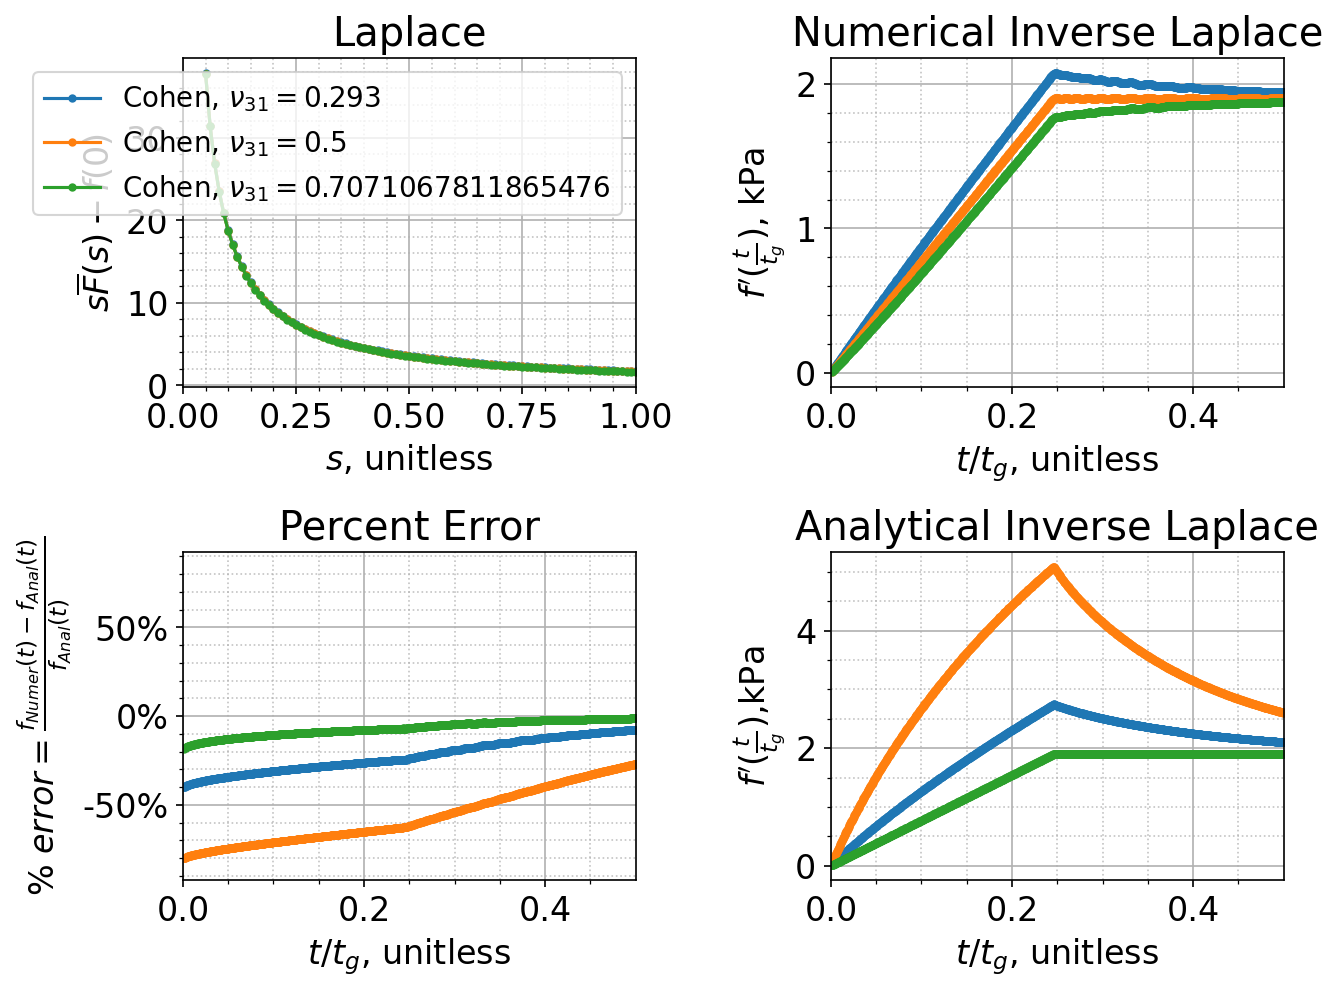
\includegraphics[width=0.66\textwidth]{PlotsWhenC1=C2.png}
\end{SCfigure}

\begin{table}[!ht]
    % https://www.tablesgenerator.com/
    \centering
    \caption{\label{tab:C1EqualsC2} Parameters for lines plotted in {Figure \ref{fig:C1EqualsC2}}}
    \tiny
    \begin{tabular}{|l|l|l|l|l|l|l|l|l|l|l|l|l|l|l|l|l|l|}
    \hline
    \rowcolor[HTML]{C0C0C0} 
        ~                        & $t_0/t_g$ & $t_g$ & $\dot{\varepsilon{}}$ & $E_1$ & $E_3$ & $\nu_{21}$ & $\nu_{31}$ & $\Delta_1$ & $\Delta_2$ & $\Delta_3$ & $C_{11}$   & $C_{12}$   & $C_{13}$ & $C_{33}$ & $C_0$  & $C_1$ & $C_2$  \\ \hline
\cellcolor[HTML]{EFEFEF}Line \#1 & 0.246184  & 40.62 & 0.01                  & 8.5   & 19    & 0.75       & 0.293      & 0.173188   & 0.549482   & 2.628      & 26.968415  & 22.111272  & 14.38    & 27.426   & 0.18   & 9.555 & 27.055 \\ \hline
\cellcolor[HTML]{EFEFEF}Line \#2 & 0.246184  & 40.62 & 0.01                  & 8.5   & 19    & 0.75       & 0.500        & 0.026316   & 0.507519   & 9.6428     & 163.928    & 159.071429 & 161.5    & 180.5    & 0.0296 & 7.823 & 7.823  \\ \hline
\cellcolor[HTML]{EFEFEF}Line \#3 & 0.246184  & 40.62 & 0.01                  & 8.5   & 19    & 0.75       & 0.707      & -0.197368  & 0.443609   & 4e-16      & -19.104762 & -23.961905 & -30.45   & -24.067  & -0.254 & 6.302 & 19.790 \\ \hline
    \end{tabular}
\end{table}

\begin{SCfigure}[0.5][!ht]  % the 0.5 represents the size of the caption relative to the figure
\centering
\caption{\label{fig:Summation_expression_only} This is the summation expression component of Cohen's analytic solution. Note that at $\nu_{31}=0.5$, the value is not uniformly $0$, and thus $f(t)$ is not proportional to $\varepsilon(t)$.}
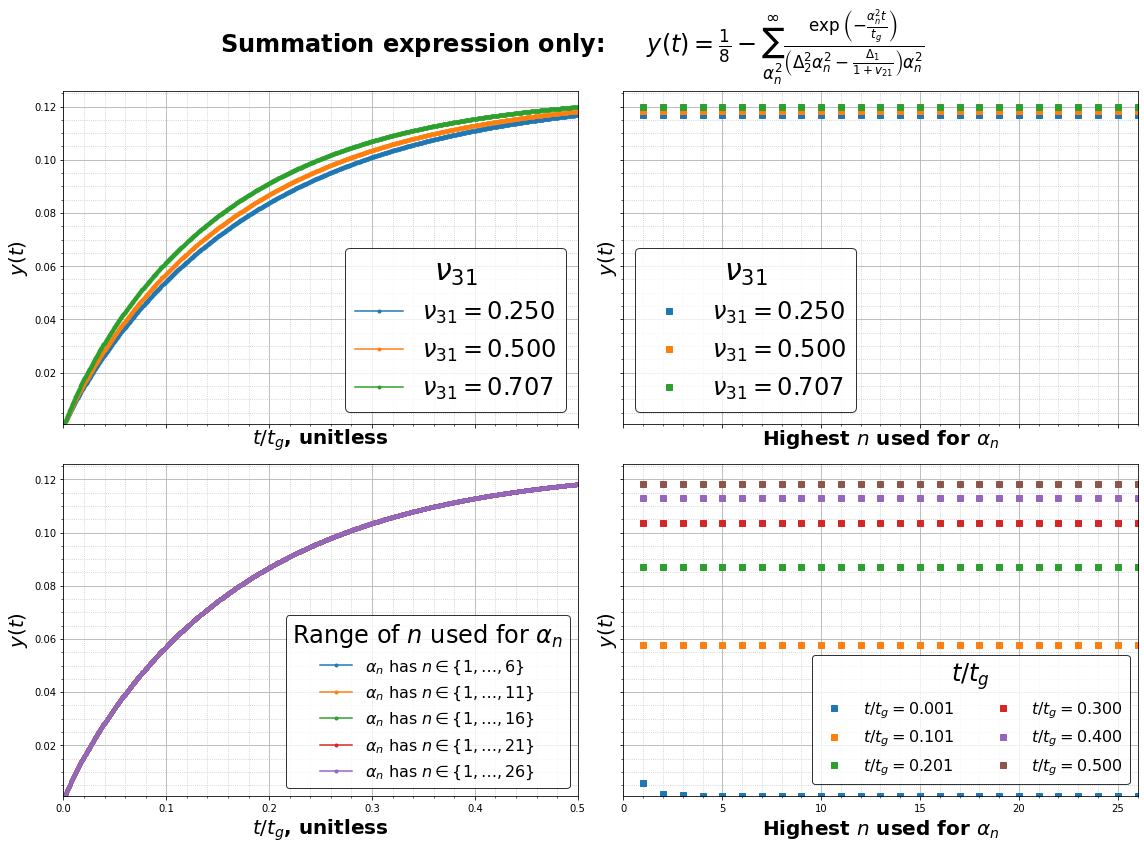
\includegraphics[width=0.66\textwidth]{Summation_expression_only.png}
\end{SCfigure}

\subsection{Proof \#1 that $C_1\!=\!C_2 \iff \nu_{31}\!=\!0.5$}

Set $C_1$ = $C_2$:
\begin{align}
\overbrace{\frac{C_{11} +C_{12} -4C_{13} +2C_{33}}{C_{11}-C_{12}}}^{C_1}
 &= \overbrace{ 2 \frac{C_{33} \left( C_{11} - C_{12} \right) + C_{11} \left( C_{11}+C_{12}-4C_{13} \right) + 2C_{13}^2 }{\left( C_{11}-C_{12} \right)^2} }^{C_2}  \\
\left( C_{11}-C_{12} \right) \left( C_{11} +C_{12} -4C_{13} +2C_{33} \right) &= 2 C_{33} \left( C_{11} - C_{12} \right) + 2 C_{11} \left( C_{11}+C_{12}-4C_{13} \right) + 4 C_{13}^2   \\
\left( C_{11}-C_{12} \right) \left( C_{11} +C_{12} -4C_{13} \right) &=  2 C_{11} \left( C_{11}+C_{12}-4C_{13} \right) + 4 C_{13}^2  \\
-\left( C_{11}+C_{12} \right) \left( C_{11} +C_{12} -4C_{13} \right) &=  4 C_{13}^2  \\
- \frac{E_1}{\Delta_1} \cdot \frac{E_1 \left(1-4\nu_{31} \right)}{\Delta_1} &= 4 \left( \frac{E_1 \nu_{31}}{\Delta_1} \right)^2 \\
\left( \frac{E_1}{\Delta_1} \right)^2 \left(4\nu_{31}-1 \right) &= 4 \nu_{31}^2 \left( \frac{E_1}{\Delta_1} \right)^2 \\
\left( 4 \nu_{31}^2 -4 \nu_{31} +1 \right) \left( \frac{E_1}{\Delta_1} \right)^2 &= 0 \\
\left( 2 \nu_{31} -1 \right)^2 \left( \frac{E_1}{\Delta_1} \right)^2 &= 0 \\
\end{align}

We know $E_1=0$ is impossible because then $C_{11}=C_{12}=0$. Thus, only solution remains: $2 \nu_{31} -1 = 0$.  \\
Therefore: 
$$\boxed{\nu_{31} = \frac{1}{2} \iff C_1=C_2}$$

\noindent\rule{20cm}{0.8pt}

\newpage 
\subsection{Proof \#2 that $C_1\!=\!C_2 \iff \nu_{31}\!=\!0.5$}
This is an alternative proof to Proof \#1.  \\
\textbf{Strategy:} Derive $C_1$ - $C_2$ directly in terms of constants ($\nu_{21}$, $\nu_{31}$, $E_1$, $E_3$), then set them equal each other.


\subsubsection{Derive $C_{11}$, $C_{12}$, $C_{13}$, and $C_{33}$ expressions directly in terms of $\nu_x$ and $E_x$ parameters}

\begin{align}
C_{11}
&=\frac{E_1 \cdot \left( 1-\nu_{31}^2 \frac{E_1}{E_3} \right)}{ \left(1+\nu_{21}\right) \cdot \Delta_1} = \textcolor{blue}{\frac{E_1 \cdot \left( 1-\nu_{31}^2 \frac{E_1}{E_3} \right)}{ \left(1+\nu_{21}\right) \left( 1-\nu_{21}-2\nu_{31}^2\frac{E_1}{E_3} \right) }} \\
C_{12} 
&=\frac{E_1 \cdot \left( \nu_{21}+\nu_{31}^2 \frac{E_1}{E_3} \right)}{ \left(1+\nu_{21}\right) \cdot \Delta_1} \textcolor{blue}{=\frac{E_1 \cdot \left( \nu_{21}+\nu_{31}^2 \frac{E_1}{E_3} \right)}{ \left(1+\nu_{21}\right)  \left( 1-\nu_{21}-2\nu_{31}^2\frac{E_1}{E_3} \right) }} \\
C_{13}
&=\frac{E_1 \nu_{31}}{ \Delta_1} \textcolor{blue}{=\frac{E_1 \nu_{31}}{ 1-\nu_{21}-2\nu_{31}^2\frac{E_1}{E_3} } }   \\
C_{33}
&=E_3 \cdot \left( 1 + \frac{  2\nu_{31}^2 \frac{E_1}{E_3}}{\Delta_1} \right)
\textcolor{blue}{ =\frac{ \Delta_1 E_3 + 2\nu_{31}^2 E_1}{\Delta_1} }  \\
& \textcolor{blue}{ =E_3 \cdot \left( 1 + \frac{  2\nu_{31}^2 \frac{E_1}{E_3}}{ 1-\nu_{21}-2\nu_{31}^2\frac{E_1}{E_3} } \right) = \frac{ \left( 1-\nu_{21}-2\nu_{31}^2\frac{E_1}{E_3} \right) E_3 + 2 \nu_{31}^2 E_1}{ 1-\nu_{21}-2\nu_{31}^2\frac{E_1}{E_3} } }  \\
& \textcolor{blue}{= \frac{ E_3 \cdot \left( 1-\nu_{21} \right) }{ 1-\nu_{21}-2\nu_{31}^2\frac{E_1}{E_3} } }  \\
\end{align}
\noindent\rule{8cm}{0.4pt}

\subsubsection{Derive combinations of $C_{11}$, $C_{12}$, etc expressions}
\textbf{Motivation}: This will make future steps (e.g. deriving $C_0$ in terms of $v_x$ and $E_x$ parameters) easier.
\begin{align}
C_{11}-C_{12}
&=\frac{E_1}{1+\nu_{21}} \\
\\
C_{11}+C_{12}
&=\frac{E_1}{\Delta_1} =\frac{E_1}{ 1-\nu_{21}-2\nu_{31}^2\frac{E_1}{E_3} } \\
\\
C_{13} 
&= \frac{E_1 \nu_{31}}{ 1-\nu_{21}-2\nu_{31}^2\frac{E_1}{E_3} }  \\
\\
C_{33} 
&= \frac{ E_3 \cdot \left( 1-\nu_{21} \right) }{ 1-\nu_{21}-2\nu_{31}^2\frac{E_1}{E_3} }  \\
\\
C_{11}+C_{12}-4C_{13} 
&= \frac{E_1 \left(1-4\nu_{31} \right)}{\Delta_1}  \\
&= \frac{E_1 \cdot \left(1-4\nu_{31} \right)}{ 1-\nu_{21}-2\nu_{31}^2\frac{E_1}{E_3} }  \\
\\
C_{11}+C_{12}-4C_{13}+2C_{33} 
&= \frac{E_1 \left(1-4\nu_{31} \right) + 2 E_3 \left( 1-\nu_{21} \right) }{ 1-\nu_{21}-2\nu_{31}^2\frac{E_1}{E_3} }  \\
&= \frac{E_1+2E_3 -4 E_1 \nu_{31} - 2E_3 \nu_{21} }{ 1-\nu_{21}-2\nu_{31}^2\frac{E_1}{E_3} }  \\
\end{align}

\noindent\rule{8cm}{0.4pt}

\subsubsection{Getting $C_0$, $C_1$, and $C_2$ directly in terms of $\nu_x$ and $E_x$ parameters}

\begin{align}
C_0 
&= \frac{C_{11} - C_{12}}{C_{11}} = \frac{\Delta_1}{1-\nu_{31}^2 \frac{E_1}{E_3}} = \frac{1-\nu_{21}-2\nu_{31}^2\frac{E_1}{E_3}}{1-\nu_{31}^2 \frac{E_1}{E_3}} \\
\\
C_1 
&= \frac{C_{11} +C_{12} -4C_{13} +2C_{33}}{C_{11}-C_{12}}   \\
&= \frac{\left( 1+\nu_{21} \right) \left( 1-4\nu_{31} + 2 \frac{E_3}{E_1} \left( 1-\nu_{21} \right) \right) }{ \left( 1-\nu_{21}-2\nu_{31}^2\frac{E_1}{E_3} \right) }  \\
\\
C_2 
&= 2 \frac{C_{33} \left( C_{11} - C_{12} \right) + C_{11} \left( C_{11}+C_{12}-4C_{13} \right) + 2C_{13}^2 }{\left( C_{11}-C_{12} \right)^2}   \\
&= 2 \frac{ \left( \frac{ E_3 \cdot \left( 1-\nu_{21} \right) }{ 1-\nu_{21}-2\nu_{31}^2\frac{E_1}{E_3} } \right) \left( \frac{E_1}{1+\nu_{21}} \right) + \left( \frac{E_1 \cdot \left( 1-\nu_{31}^2 \frac{E_1}{E_3} \right)}{ \left(1+\nu_{21}\right) \left( 1-\nu_{21}-2\nu_{31}^2\frac{E_1}{E_3} \right) } \right)  \left( \frac{E_1 \cdot \left(1-4\nu_{31} \right)}{ 1-\nu_{21}-2\nu_{31}^2\frac{E_1}{E_3} } \right) + 2 \left( \frac{E_1 \nu_{31}}{ 1-\nu_{21}-2\nu_{31}^2\frac{E_1}{E_3} } \right)^2 }{\left( \frac{E_1}{1+\nu_{21}} \right)^2}   \\
&= 2 \frac{ E_3 E_1 \left( 1-\nu_{21} \right) \left( 1-\nu_{21}-2\nu_{31}^2\frac{E_1}{E_3}  \right) + E_1^2 \cdot \left( 1-\nu_{31}^2 \frac{E_1}{E_3} \right) \left(1-4\nu_{31} \right)+ 2 E_1^2 \nu_{31}^2 \left( 1+\nu_{21} \right) }{\left( \frac{E_1}{1+\nu_{21}} \right)^2 \left( 1-\nu_{21}-2\nu_{31}^2\frac{E_1}{E_3} \right)^2 \left( 1+\nu_{21} \right) }   \\
&= 2 \frac{ \frac{E_3}{E_1} \left( 1-\nu_{21} \right) \left( 1-\nu_{21}-2\nu_{31}^2\frac{E_1}{E_3}  \right) + \left( 1-\nu_{31}^2 \frac{E_1}{E_3} \right) \left(1-4\nu_{31} \right)+ 2\nu_{31}^2 \left( 1+\nu_{21} \right) }{ \frac{ \left( 1-\nu_{21}-2\nu_{31}^2\frac{E_1}{E_3} \right)^2 }{1+\nu_{21}} }   \\
&= 2 \frac{ \frac{E_3}{E_1} \left( 1-\nu_{21}^2 \right) \left( 1-\nu_{21}-2\nu_{31}^2\frac{E_1}{E_3}  \right) + \left( 1-\nu_{31}^2 \frac{E_1}{E_3} \right) \left(1-4\nu_{31} \right) \left(1+\nu_{21}\right) + 2\nu_{31}^2 \left( 1+\nu_{21} \right)^2 }{ \left( 1-\nu_{21}-2\nu_{31}^2\frac{E_1}{E_3} \right)^2 }   \\
&= 2 \left( 1+\nu_{21} \right) \frac{ \frac{E_3}{E_1} \left( 1-\nu_{21} \right) \left( 1-\nu_{21}-2\nu_{31}^2\frac{E_1}{E_3}  \right) + \left( 1-\nu_{31}^2 \frac{E_1}{E_3} \right) \left(1-4\nu_{31} \right)+ 2\nu_{31}^2 \left( 1+\nu_{21} \right) }{ \left( 1-\nu_{21}-2\nu_{31}^2\frac{E_1}{E_3} \right)^2 }   \\
\end{align}


\noindent\rule{8cm}{0.4pt}

\subsubsection{Solve for $C_1$=$C_2$}
Knowing:
\begin{align}
C_0 &= \frac{1-\nu_{21}-2\nu_{31}^2\frac{E_1}{E_3}}{1-\nu_{31}^2 \frac{E_1}{E_3}} \\
\\
C_1 &= \frac{\left( 1+\nu_{21} \right) \left( 1-4\nu_{31} + 2 \frac{E_3}{E_1} \left( 1-\nu_{21} \right) \right) }{ 1-\nu_{21}-2\nu_{31}^2\frac{E_1}{E_3} }  \\
\\
C_2 
&= 2 \frac{ \frac{E_3}{E_1} \left( 1-\nu_{21}^2 \right) \left( 1-\nu_{21}-2\nu_{31}^2\frac{E_1}{E_3}  \right) + \left( 1-\nu_{31}^2 \frac{E_1}{E_3} \right) \left(1-4\nu_{31} \right) \left(1+\nu_{21}\right) + 2\nu_{31}^2 \left( 1+\nu_{21} \right)^2 }{ \left( 1-\nu_{21}-2\nu_{31}^2\frac{E_1}{E_3} \right)^2 }   \\
\end{align}

We want to solve for $C_1$=$C_2$:

\begin{align*}
\overbrace{\frac{\left( 1+\nu_{21} \right) \left( 1-4\nu_{31} + 2 \frac{E_3}{E_1} \left( 1-\nu_{21} \right) \right) }{ 1-\nu_{21}-2\nu_{31}^2\frac{E_1}{E_3} } }^{C_1}
&= 
\overbrace{
2 \frac{
    \scriptstyle{
\frac{E_3}{E_1} \left( 1-\nu_{21}^2 \right) \left( 1-\nu_{21}-2\nu_{31}^2\frac{E_1}{E_3}  \right) + \left( 1-\nu_{31}^2 \frac{E_1}{E_3} \right) \left(1-4\nu_{31} \right) \left(1+\nu_{21}\right) + 2\nu_{31}^2 \left( 1+\nu_{21} \right)^2}
}{
\left( 1-\nu_{21}-2\nu_{31}^2\frac{E_1}{E_3} \right)^2 
} }^{C_2}  \tag{A}  \\
\end{align*}

Multiply both sides by $\left( 1-\nu_{21}-2\nu_{31}^2\frac{E_1}{E_3} \right)^2$
\begin{align*} 
\left( 1+\nu_{21} \right) \left( 1-4\nu_{31} + 2 \frac{E_3}{E_1} \left( 1-\nu_{21} \right) \right)  \left( 1-\nu_{21}-2\nu_{31}^2\frac{E_1}{E_3}  \right)
=&  2 \frac{E_3}{E_1} \left( 1-\nu_{21}^2 \right) \left( 1-\nu_{21}-2\nu_{31}^2\frac{E_1}{E_3}  \right) \\
&+ 2 \left( 1-\nu_{31}^2 \frac{E_1}{E_3} \right) \left(1-4\nu_{31} \right) \left(1+\nu_{21}\right)  \\
&+ 4\nu_{31}^2 \left( 1+\nu_{21} \right)^2   \\
\small{\text{Divide both sides by }}&\scriptscriptstyle{1+\nu_{21}}
\\ 
{\left( 1-4\nu_{31} + 2 \frac{E_3}{E_1} \left( 1-\nu_{21} \right) \right)  \left( 1-\nu_{21}-2\nu_{31}^2\frac{E_1}{E_3}  \right) }
=& 
2 \frac{E_3}{E_1} \left( 1-\nu_{21} \right) \left( 1-\nu_{21}-2\nu_{31}^2\frac{E_1}{E_3}  \right) \\
&+ 2\left( 1-\nu_{31}^2 \frac{E_1}{E_3} \right) \left(1-4\nu_{31} \right) + 4\nu_{31}^2 \left( 1+\nu_{21} \right) 
\tag{B} \\
\left( 1-4\nu_{31} \right)  \left( 1-\nu_{21}-2\nu_{31}^2\frac{E_1}{E_3}  \right)
=&
\underbrace{2\left( 1-\nu_{31}^2 \frac{E_1}{E_3} \right) \left(1-4\nu_{31} \right)}_{\text{Move to lefthand side}} + 4\nu_{31}^2 \left( 1+\nu_{21} \right) 
\tag{C} \\
\left( 1-4\nu_{31} \right)  \left( 1-\nu_{21}-2\nu_{31}^2\frac{E_1}{E_3} -2\left( 1-\nu_{31}^2 \frac{E_1}{E_3} \right) \right)
=&
4\nu_{31}^2 \left( 1+\nu_{21} \right) 
\tag{D} \\
\left( 1-4\nu_{31} \right)  \left( -1- \nu_{21}\right) =& 4\nu_{31}^2 \left( 1+\nu_{21} \right) 
\tag{E} \\
-\left( 1-4\nu_{31} \right) \left(1+\nu_{21}\right)  &= 4\nu_{31}^2 \left( 1+\nu_{21} \right)  
\tag{F} \\
-\left( 1-4\nu_{31} +4\nu_{31}^2 \right) \left(1+\nu_{21}\right)  =& 0 
\tag{G}  \\
-\left( 4\nu_{31}^2-4\nu_{31}+1 \right) \left(1+\nu_{21}\right)  =& 0 
\tag{H} \\
-\left( 2\nu_{31}-1 \right)^2 \left(1+\nu_{21}\right)  =& 0   
\tag{I} \\
-\left( 2\nu_{31}-1 \right)^2 \left(1+\nu_{21}\right)  =& \left( C_1-C_2 \right) \overbrace{ \times \frac{\left( 1-\nu_{21}-2\nu_{31}^2\frac{E_1}{E_3}  \right)^2}{ 1+\nu_{21} } }^{\text{Multiplications/divisions } \text{done to get to this step}} \\
-\frac{ \left( 2\nu_{31}-1 \right)^2 \left(1+\nu_{21}\right)^2 }{\left( 1-\nu_{21}-2\nu_{31}^2\frac{E_1}{E_3}  \right)^2} =& C_1-C_2   
\end{align*}



\begin{gather*}
\boxed{
C_2-C_1 = \left( \frac{ \left( 2\nu_{31}-1 \right) \left(1+\nu_{21}\right) }{1-\nu_{21}-2\nu_{31}^2\frac{E_1}{E_3}  } \right)^2    }
\tag{J} \\
\end{gather*}



\text{Since }  $\nu_{21}\!=\!-1 \implies C_{11} \text{ and } C_{12}$ \text{ are undefined, } \text{we know $C_{11}=C_{12}$ has only one solution remaining: }


\boxed{
C_1=C_2 \iff \nu_{31}=0.5 \\
\text{\qquad assuming } 1-\nu_{21}-2\nu_{31}^2\frac{E_1}{E_3} \neq 0
} 
\\
\noindent\rule{8cm}{0.4pt}

\printbibliography


\end{document}